\documentclass{ML}
\usepackage{amssymb}
\usepackage{algorithm}
\usepackage{float}
\usepackage[noend]{algpseudocode}
\usepackage{amsmath}
\newtheorem{theorem}{\hspace{2em}定理}
\newtheorem{lemma}{Lemma}
\usepackage{xinttools} % for the \xintFor***
\usepackage{tikz}
\usetikzlibrary{calc}


\def\biglen{20cm} % playing role of infinity (should be < .25\maxdimen)
% define the "half plane" to be clipped (#1 = half the distance between cells)
\tikzset{
  half plane/.style={ to path={
       ($(\tikztostart)!.5!(\tikztotarget)!#1!(\tikztotarget)!\biglen!90:(\tikztotarget)$)
    -- ($(\tikztostart)!.5!(\tikztotarget)!#1!(\tikztotarget)!\biglen!-90:(\tikztotarget)$)
    -- ([turn]0,2*\biglen) -- ([turn]0,2*\biglen) -- cycle}},
  half plane/.default={1pt}
}

\def\n{2} % number of random points
\def\maxxy{6} % random points are in [-\maxxy,\maxxy]x[-\maxxy,\maxxy]
\def\maxy{3}
\makeatletter
\newenvironment{breakablealgorithm}
  {% \begin{breakablealgorithm}
   \begin{center}
     \refstepcounter{algorithm}% New algorithm
     \hrule height.8pt depth0pt \kern2pt% \@fs@pre for \@fs@ruled
     \renewcommand{\caption}[2][\relax]{% Make a new \caption
       {\raggedright\textbf{\ALG@name~\thealgorithm} ##2\par}%
       \ifx\relax##1\relax % #1 is \relax
         \addcontentsline{loa}{algorithm}{\protect\numberline{\thealgorithm}##2}%
       \else % #1 is not \relax
         \addcontentsline{loa}{algorithm}{\protect\numberline{\thealgorithm}##1}%
       \fi
       \kern2pt\hrule\kern2pt
     }
  }{% \end{breakablealgorithm}
     \kern2pt\hrule\relax% \@fs@post for \@fs@ruled
   \end{center}
  }
  \makeatother
% 姓名,学号
\infoauthor{1160300312\ 靳贺霖}{1160300314\ 朱明彦}

% 课程类型,实验名称
\infoexp{课程类型}{分布式空间近似关键字查询系统}

\infoschool{计算机学院}{杨东华、王金宝}

\begin{document}
\maketitle

\tableofcontents
\newpage

\begin{center}
  \textbf{\zihao{3} 分布式空间近似关键字查询系统}
\end{center}

\section{问题描述}
\subsection{数据}\label{sec:data}
空间对象集合$D = \{o_1, o_2, \dots, o_n\}$,对于$D$中任意一个对象$o_i = (loc_i, kw_{i, 1}, \dots, kw_{i, m})$,
即包含$\mathbb{R}^d$维欧式空间中一个点$loc_i$和一组关键字$kw_{i, 1}, \dots, kw_{i, m}$,记为$o_i.loc = loc_i$和$o_i.kw = \{kw_{i, 1}, \dots, kw_{i, m}\}$。
\textbf{在本项目中主要针对$d = 2$的情况,$\mathbb{R}^2$对于现实中的应用有着很大的价值。}

\subsection{范围查询}\label{sec:range-query}
\paragraph{输入:}$Q = (Q_{rs}, Q_{rt})$,其中$Q_{rs}$是一个空间范围($\mathbb{R}^d$维欧式空间中的超立方体);$Q_{rt}$为关键字近似条件,
$Q_{rt} = \{(kw_1, \theta_1), \dots, (kw_K, \theta_K)\}$,其中$\theta_i$为阈值。
\paragraph{输出:}$O = \{o | o \in D, o.loc \in Q.Q_s, \forall(kw_i, \theta_i) \in Q.Q_t, \exists o.kw_j, \mathrm{ED}(kw_j, kw_i) \leq \theta_i\}$,
其中$\mathrm{ED}(kw_j, kw_i)$表示两个关键字$kw_j$和$kw_i$之间的编辑距离。

\subsection{$k$NN查询}\label{sec:knn_query}
\paragraph{输入:} $Q = (Q_s, Q_t, k)$,其中$Q_s = loc$是$\mathbb{R}^d$维欧式空间中一个点,即查询发出的位置;
$Q_t = \{(kw_1, \theta_1), \dots, (kw_K, \theta_K)\}$;$k$为表示最近邻居的数量。
\paragraph{输出:}对$O_t = \{o | o \in D, \forall(kw_i, \theta_i) \in Q.Q_t, \exists o.kw_j, \mathrm{ED}(kw_j, kw_i) \leq \theta_i\}$,
根据$|O_t|$的大小进行定义,
\begin{itemize}
    \item 如果$|O_t| \leq k$,则$O_{k\mathrm{NN}} = O_t$即为最终结果。
    \item 如果$|O_t| > k$,$O_{k\mathrm{NN}}= \{o | o \in O_t, \forall o_i \in O_t - O, \mathrm{Dis}(loc, o_i) \ge \mathrm{Dis}(loc, o_j)$对$\forall o_j \in O$成立$\}$
    并且$|O_{k\mathrm{NN}}| = k$。
\end{itemize}

\subsection{Reverse $k$NN查询}\label{sec:RkNN-query}
\paragraph{输入:}与\ref{sec:knn_query}节输入相同,不再赘述。
\paragraph{输出:}$O_{\mathrm{R}k\mathrm{NN}} = \{o_{R_1}, \dots, o_{R_M}\}$,对于$O_{\mathrm{R}k\mathrm{NN}}$中的任一元素$o_{R_i}$
均有$o_{k\mathrm{NN}} \in O_{R_i-k\mathrm{NN}}$且$o_{R_i} \in D$,其中$o_{k\mathrm{NN}}.loc = Q_s, o_{k\mathrm{NN}}.kw = Q_t$;$O_{R_i-k\mathrm{NN}}$是以$(o_{R_i}.loc, o_{R_i}.kw, k)$为输入的$k$NN查询结果。
% \section{系统设计}
% 存储、索引、算法(建议加入系统架构图、设计示例)

\newpage
% TODO 注意仅用于记录思路,提交时删除。
主要思路\begin{itemize}
    \item 存储部分,类似Spark、HDFS进行处理
    \item 索引和算法部分,两层索引结构,组织不同节点间的索引使用\texttt{RT-CAN}\cite{RT-CAN},在本地使用以R树为核心,结合MHR-Tree\cite{MHR-Tree}
    进行范围查询,结合Voronoi Diagrams\cite{VoR-Tree}进行$k$NN查询和Reverse $k$NN查询。
\end{itemize}

\section{Background}
\subsection{R-Tree}
R-Tree\cite{R-Tree}是如今处理空间查询最常用的索引,它将$\mathbb{R}^d$中的数据
划分到$d$维超立方体(Minimum Bounding Rectangle),并将每个超立方体存储在叶子节点。
将每个数据划分到叶子后,再递归地寻找MBR能够覆盖若干个叶子,直到仅剩一个MBR,即为R-Tree的根节点。

\subsection{Voronoi图}
Voronoi Diagram\cite{Voronoi-Diagram}是一种根据点之间特定的距离度量方式将空间划分成若干区域的划分方式。
对于$\mathbb{R}^d$中的一个集合$D = \{p_1, p_2, \dots, p_n\}$上的Voronoi图,将$\mathbb{R}^d$划分为$n$
个区域,每个区域中包含着距离$D$中某一个数据在$\mathbb{R}^d$最近的所有点,其中距离$\mathrm{Dis}(.,.)$的定义方式可以自行给定。

换而言之,如果给定$q \in \mathbb{R}^d, p_i \in D$,如果$q$在Voronoi图中包含$p_i$的区域里,则
$$\forall j \neq i, p_j \in D, \mathrm{Dis}(p_j, q) \ge \mathrm{Dis}(p_i, q)$$
由上述性质以及在\cite{VD-Property}中提到的性质,Voronoi图在处理$k$NN查询和Reverse $k$NN查询有着很好的效果。
\textbf{在本项目中,主要关注$d = 2$并且使用欧式距离度量的情况。}

\subsection{MHR-Tree}
MHR-Tree\cite{MHR-Tree}本质上是在R树上增加关键字集合的信息(min-hash签名),并使用基于$q$-gram集合
的剪枝策略来处理近似关键字的条件。从根节点开始的查询,根据查询关键字$\sigma$和某一个内节点$u$的
$q$-gram集合$|g_{\sigma} \cap g_u|$的大小来进行剪枝。
\begin{itemize}
    \item 当$|g_{\sigma} \cap g_u| < |\sigma| - 1 - (\tau - 1) * q$时,无需访问$u$,其中$\tau$为编辑距离的阈值。
    \item 否则,需要访问内节点$u$。
\end{itemize}
而根据\cite{MHR-Tree}中可以通过$s(g_{\sigma})$和$s(g_{u})$来估计$|g_{\sigma} \cap g_u|$,主要依赖于下式
$$ \widehat{|g_{\sigma} \cap g_u|} = \hat{\rho}(g_{\sigma}, g_u) \times \widehat{|g_{\sigma} \cup g_u|}$$

\subsection{CAN}
CAN(Content Addressable Network)是一种自组织性很强的P2P覆盖网络,一个$d$维的CAN的划分是将一个$d$维的坐标系划分到不同的节点上去。数据是通过一个$hash$函数来将数据的主键划分为$d$维的坐标,从而划分数据到不同的CAN节点上的。对于一个CAN节点$N_i$来说,它会保存所有和$N_i$对应的空间的邻接空间的ip地址,从而形成一个P2P网络。因为CAN网络的自组织性很强,所以一个节点可以很自由地加入或者离开一个CAN,就像P2P网络一样,只需要发送信息更改网络拓扑即可。

我们使用的RT-CAN索引的构建是基于一种CAN的变种,$C^2$来实现的。$C^2$除了有CAN的特征外,它还在划分坐标系的每个维度上添加了和弦邻居链接(Chord-like neighbor link)。具体而言,在每个维度上距离为$2^0,2^1,\cdots$的节点上添加链接。因为我们要实现的是分布式空间近似关键字查询,所以我们选择中2维的$C^2$来实现的RT-CAN索引。

我们要处理的是空间近似关键字查询以及$k$NN,R$k$NN近似关键字查询,所以我们的数据的key值就可以看作是2维的位置坐标,这样很自然的就可以想到对CAN的划分也是在2维坐标中而且可以和位置信息对应起来,即$hash$函数不对输入进行转换。

\section{存储}
\subsection{数据划分}\label{sec:data-partition}
数据的划分我们使用的是一种类似于KD树划分的方法。我们知道\cite{KD-Tree-Partition},KD树有一种划分的算法按照如下的方法进行:
\begin{enumerate}
  \item 从方差最高的维度开始,并按照这个维度的数据值对空间进行划分,一般取方差最高的那个维度的值的中值作为划分值;
  \item 重复在下一个方差最高的维度继续进行划分,直到空间被划分成想要的份数。 
\end{enumerate}
我们的划分和这种对KD树的划分有所不同。对于分布式系统,我们更关心的是每个计算节点的数据分配和负载平衡,所以我们对其作一定的修改。首先,设置一个阈值参数$P_{max}$,然后按照如下的方法进行划分:
\begin{enumerate}
  \item 判断数据点的数量是否小于$P_{max}$,如果小于则无需划分。否则找到数据中方差最高的维度,按照这个维度的中值作为划分值划分数据;
  \item 重复对每一个数据点个数大于$P_{max}$的块进行划分:找到块中方差最高的维度,按照这个维度的中值作为划分值划分这个块。 
\end{enumerate}
这样,我们就能保证每个块中的数据点数量不少于$P_{max}/2$而且不多于$P_{max}$,保证了一定的负载均衡而且保证数据量不超过阈值$P_{max}$,防止节点负载过大。当数据量大的时候可以选择尽可能较大的$P_{max}$充分利用每个节点的存储计算性能;当数据量小的时候可以适量调小$P_{max}$以便数据更分散地分配到各个节点中提高并行性。
\subsection{数据备份}
为了使系统有一定的对抗异常状态的容错能力,数据备份是必不可少的,这里我们选择使用primary-secondary的中心副本控制协议来实现数据的备份并维护副本之间的一致性。在primary-secondary协议中,副本被分为两类,其中有一个副本被当作primary副本,它是中心节点,负责维护数据的更新,并发控制以及维护副本之间的一致性等。其他的副本都是secondary副本。

如图2所示,数据更新的过程中,外部的节点发送请求给primary节点,然后primary节点再将更新操作分发给所属它的secondary节点。这个过程我们选择提供最终一致性,即secondary节点和primary节点不一致,需要的只是后续过程中secondary节点能够可以同步到primary一致的状态即可。但是可能发生的问题就是secondary未与primary更新一致的情况下primary节点又收到了一个更新请求,会产生不一致的情况。对于这种情况,我们选择在secondary节点同步到和primary节点过程中,secondary节点同步到primary某个时刻的快照(snapshot)的状态,更新完如果仍不一致则继续更新。

数据更新过程中由于secondary节点的数据可能会落后于primary节点,所以一些存储“旧”数据的secondary节点的部分数据其实是不可用的。为了解决这个问题,我们将secondary节点的状态分为两种:一种是与primary一致的状态,这时可以读取其中的数据;另一种是被标记为不可用的状态,表明secondary节点的数据仍处于被更新的状态从而无法读取其中的数据。从某种意义上来讲,这种方法通过降低了一定的可用性来提高系统的一致性。

primary节点宕机后,选择合适的primary副本进行替换也是很重要的一个问题。和更新类似,选择一个状态为和primary节点一致的secondary节点替换primary节点即可。但是可能存在的状态是所有的secondary节点都恰好是不可用的状态,对于这种情况,我们选择通过日志来对secondary的记录进行恢复。设置检查点(checkpoint),在检查点之后将secondary节点的数据利用日志记录进行更新,使其成为primary节点宕机前的状态即可。

\section{两层索引结构}
\subsection{全局索引(RT-CAN)}
我们使用RT-CAN索引作为我们的第一层索引,即寻找存储节点的索引。RT-CAN索引是一种建立在本地索引之上的索引\cite{RT-CAN}。
它使用$C^2$网络作为底层存储节点分布,通过定义R树数据节点如何划分到各个存储节点来得到数据的组织方式,并且定义相关算法能对其中的数据进行查询。
下面首先介绍RT-CAN节点的结构,然后介绍如何构造RT-CAN索引。

\subsubsection{RT-CAN节点结构}
RT-CAN索引是建立在一个shared-nothing的集群上的。
如图1所示,集群中的每一个节点$N_i$都包含了两个部分:一个是存储节点$N_{si}$,另一个是覆盖节点$N_{oi}$。
$N_{si}$表示的是分布式存储的特征,它存储着所有数据划分的一部分。
为了满足空间近似查询,以及空间近似的$k$NN和R$k$NN查询,$N_{si}$使用了一种R树的变种来存储局部数据,从而满足我们的查询需求。
$N_{oi}$是用来表示CAN结构化覆盖的部分,它负责的是CAN划分的一部分。
对于CAN的网络通信来说,$N_{si}$会适应性的选择一部分局部R树的结点,然后通过$N_{oi}$来将这些节点信息发送到CAN网络中。
发送的信息结果为一个二元组$(ip,mbr)$,其中ip是$N_i$节点的IP地址,$mbr$是这个R树结点的范围。
当$N{si}$收到$N_{oi}$的发送请求时,$N{si}$就会选择相应的R树结点并将其map成为一个CAN节点,并通过CAN的路由协议将请求发出。
$N_{oi}$维护着全局索引,当它收到一个广播请求,它就通过map方法判断这是否是它要接受的请求。
如果时,它就保留一份广播的R树的结点当作索引并保存。这样就能做到用一些R树的结点来当作索引并将其分布在集群中。

\subsubsection{RT-CAN索引构造}
基于我们的需求,我们使用的是二维的$C^2$来构建我们的RT-CAN索引。
前面提到我们需要一个map方法将一个R树结点map为一个CAN节点,这样的map方法一般要以这个R树节点的中心和半径来确定。
对一个二维的R树节点$n$,范围为$[l_1,u_1],[l_2,u_2]$,中心和半径分别表示为$c_n=(\frac{l_1+u_1}{2}),r_n=\frac{1}{2}\sqrt{(u_1-l_1)^2+(u_2-l_2)^2}$。
首先,对于R树节点$n$,我们首先把它map到包含$n$的中心$c_n$的CAN节点$N_c$上,然后$N_c$会比较$n$半径和定义的一阈值参数$R_{max}$,
如果$n$的半径小于$R_{max}$,就只需要map给这一个CAN节点,否则就需要将$n$发送给所有和$n$范围覆盖的所有CAN节点。
这样可能会导致一些副本的出现,但同时也会提升查询的效率,因为只保存一个索引会导致所有相关的搜索都要在网络中查询这个索引,会降低查询效率。

然后,对于索引的构造,对于每个CAN节点,若假设其存储的R树是$L$层的,我们就选择将R树的$L-1$层的所有R树节点发送,因为它们不是经常被更新的,这样就减少了更新索引的次数。然后对每个CAN节点都执行发送的操作,然后就可以按照我们前面提到的map算法来判断如何构造我们的全局索引。

\subsubsection{RT-CAN的性质}
\begin{theorem}\label{theorem:RT-CAN-1}
  对一个点查询$Q(key)$,如果我们查询了所有以$key$为圆心,$R_{max}$为半径的的圆覆盖的所有的CAN,那么我们就一能得到完整的结果。
\end{theorem}

\begin{theorem}\label{theorem:RT-CAN-2}
  对于一个范围查询$Q(range)$,如果我们查询了所有以$range$的中心为圆心,$R_{max}+range.radius$为半径的源覆盖的所有的CAN,那么我们就一定能得到完整的结果。
\end{theorem}

\subsection{本地索引(\textit{MVR-Tree})}
本地索引结构主要是基于R-Tree\cite{R-Tree},结合\cite{MHR-Tree}和\cite{VoR-Tree}两篇文章的工作,
分别取MHR-Tree在处理范围查询上的良好表现,以及Voronoi图在处理$k$NN和R$k$NN上的良好效果,
所以将本地的索引结构称为\textit{\textbf{MVR-Tree}(\textbf{M}in-wise signature with linear hashing and \textbf{V}oronoi diagram \textbf{R-Tree})}。

由RT-CAN给每个单机分配的内容,我们可以得到的一个R树;% todo 通顺
根据\cite{VD-Property}中提到的如Fortune's sweepline算法,可以用来构建$D$上的
Voronoi图,并将Voronoi图中的邻居$VN(o_i)$和每个cell对应的区域$V(o_i)$记录在每个节点$o_i$中;
另外根据R树每个叶子节点$o_i$的关键字信息,可以计算其对应的$q$-grams $g_{o_i}$和对应的min-hash签名$s(g_{o_i})$,
并根据所有叶子节点的$s(g_{o_i})$可以递归地自底向上的构建出所有R树内节点的min-hash签名\cite{MHR-Tree}。

因此,\textbf{\textit{MVR-Tree}是一个R树的变种,并在每个叶子节点$o_i$记录Voronoi图的信息$VN(o_i), V(o_i)$和
min-hash信息$g_{o_i}, s(g_{o_i})$,以及在每个内节点$u$记录$s(g_u)$。}

\subsection{二级索引维护}\label{sec:maintain-index}
数据的插入和删除最终都可以定位到局部R树的插入和删除,从而可能会引起一些R树节点发生变化。如果引起变化的结点是已经发送到全局索引的节点的话,这时候就会产生一部分的“脏”索引,通过这些索引查找结果很可能会将查找引导到不正确的存储节点上。

为了解决这个问题,对于已经发送到全局作为索引的R树结点$n_{old}$,会给其一个标记表示这个节点已被发送到全局索引。如果插入和删除动作导致$n_{old}$分割或者合并的话,我们需要重新将这个新的R树节点集合$S_{new}$发送,从而替代之前发送的已经
过时的索引。替代过程分删除源索引和添加新索引两部分。因为$n_{old}$和$S_{new}$中各结点的中心和半径不同,所以要按$n_{old}$的中心和半径发布删除信息将旧的索引结点全都删除;然后对于$S_{new}$中的各个节点,按照它们的中心和半径发送索引消息作为新的全局索引存储即可。
\section{查询处理}
在本地使用MVR-Tree进行范围查询、$k$NN查询和R$k$NN查询,分别是使用\cite{MHR-Tree}
中针对range query的方法和使用\cite{VoR-Tree}中针对$k$NN和R$k$NN的方法来实现。

\textbf{可以这样做的正确性是依赖于R树的性质:无论是\cite{MHR-Tree}中提出的MHR-Tree和\cite{VoR-Tree}中
提出的VoR-Tree,都是在叶子节点增加了额外的信息用于查询式剪枝,而没有改变R树的性质。并且在\cite{VoR-Tree}中
提到所有原本在R树上可以进行的查询,都可以在VoR-Tree上照常进行。而MVR-Tree只是结合了两种索引,并没有改变
本质上作为R树的性质。所以直接利用\cite{MHR-Tree}和\cite{VoR-Tree}中的相应算法,在MVR-Tree上就可以进行查询,并且可以保证正确性}。

\subsection{Range Query}
对于\ref{sec:range-query}节所提到的范围查询,$1-8$行根据\cite{RT-CAN}中Range Query的方式
将查询定位到若干台机器上,$9-27$行是在本地利用MVR-Tree进行查询。其中通过$14-15$行来实现近似关键字查询剪枝;
通过12行来实现范围上的查询。具体的步骤见算法\ref{alg:range-query}。
\begin{breakablealgorithm}
  \caption{Range Query(RT-CAN $Root$, $(Q_{rs}, Q_{rt})$)}
  \label{alg:range-query}
  \begin{algorithmic}[1]
    \State $S_t = \emptyset$
    \State $N_{init} = CAN.lookup(Q_{rs}.center)$ \Comment{$Q_{rs}.center$是查询范围$Q_{rs}$的中心}
    \State $C = generateSearchCircle(Q_{rs}.center, R_{max} + Q_{rs}.radius)$ \Comment{$Q_{rs}.radius$根据定理\ref{theorem:RT-CAN-2}计算}
    \For{i = 1 to $d$}
    \State 将$C$根据$l_i, u_i$划分为$R_0, R_1, R_2$
    \State $C = R_0$
    \State 将查询信息发送到$N_1, N_2$在上面重复该查询 \Comment{$N_1, N_2$是$N_{init}$的邻居}
    \EndFor
    \State $S_i = N_{init}.globalIndex$
    \For{$\forall I \in S_i$}
    \If{$I$的区域与$Q_{rs}$有交集}
    \State 利用$I$找到本地MVR-Tree索引$R$
    \State 将队列$L$和本地结果$O$初始化为$\emptyset$
    \State 将$R$的根节点$u$插入$L$
    \While{$L \neq \emptyset$}
    \State 取$L$的队首元素$u$并且其弹出
    \If{$u$是叶节点}
    \For{对于每个$o \in u$}
    \If{$o$在$Q_{rs}$中 \textbf{and} $|g_o \cap g_{\sigma}| \ge \max(|kw_i|, |kw_j|) - 1 - (\theta_j - 1) * q$}
    \If{$\mathrm{ED}(kw_i, kw_j) < \theta_j$}\Comment{$kw_i \in o.kw, (kw_j, \theta_j) \in Q_{rt}$}
    \State 将$o$插入$O$中
    \EndIf
    \EndIf
    \EndFor
    \Else
    \For{$u$的每个子节点$p_i$}
    \If{$Q_{rs}$和$p_i$的区域存在交集}
    \State 利用\cite{MHR-Tree}中提到的方法估计$\widehat{|g_{kw_i} \cap g_{kw_j}|}$
    \Comment{$g_{kw_i}$是$p_i$节点关键字的min-hash签名}
    \If{$\widehat{|g_{kw_i} \cap g_{kw_j}|} \ge |kw_j| - 1 - (\theta_j - 1) * q$}
    \State 将$p_i$插入$L$中
    \EndIf
    \EndIf
    \EndFor
    \EndIf
    \EndWhile
    \State 输出$O$
    \EndIf
    \EndFor
  \end{algorithmic}
\end{breakablealgorithm}

\subsection{$k$NN Query}\label{sec:algo-knn}
对于\ref{sec:knn_query}节提到的$k$NN查询,是利用MVR-Tree先找到距离查询$Q_s$最近的邻居(即$1$NN),
根据$1$NN的结果以及其在Voronoi图上的邻居来实现接下来查询的剪枝,如此相比\cite{MHR-Tree}中直接利用MHR-Tree和
堆进行的$k$NN查询具有更好的I/O代价\cite{VoR-Tree}。具体的过程如算法\ref{alg:1nn-query}和\ref{algo:knn-query}所示。
\begin{breakablealgorithm}
  % TODO 对于1NN而言同样有可能跨机器,如何处理跨机器仍然是一个待做项目。
    \caption{$1$NN Query(RT-CAN $Root$, $(Q_{s}, Q_{t}, k)$)}
    \label{alg:1nn-query}
    \begin{algorithmic}[1]
      \State 根据$Q_s$将查询定位到某一台机器$N$上,得到$N$上MVR-Tree根节点$R$
      \State 将小顶堆$H$初始化为$\emptyset$,$bestDist = \infty$,$bestNN = null$
      \State 将$R$的根节点$r$插入$H$,即$H = \{(r, 0)\}$
      \While{$H \neq \emptyset$}
      \State 取$H$的堆顶元素$u$并且其弹出
      \If{$u$是叶节点}
      \For{对于每个$o \in u$}
      \If{$\mathrm{Dis}(Q_s, o) < bestDist$}
      \State $bestNN = o; bestDist = \mathrm{Dis}(Q_s, o)$
      \EndIf
      \EndFor
      \If{$bestNN != null$ \textbf{and} $V(bestNN)$ 包含 $o$}
      \State \textbf{Break;}
      \EndIf
      \Else
      \For{$u$的每个子节点$p_i$}
      \State 将$(p_i, mindist(p_i, Q_s))$插入$H$中
      \EndFor
      \EndIf
      \EndWhile
    \end{algorithmic}
  \end{breakablealgorithm}

  \begin{breakablealgorithm}
    \caption{$k$NN Query(MVR-Tree $R$, $bestNN$, ($Q_s, Q_t, k$), $counter$)}
    \label{algo:knn-query}
    \begin{algorithmic}[1]
      \If{$bestNN != null$}
      \State 将小顶堆$H$初始化为$\emptyset$
      \State 将$H$弹空,将$(bestNN, \mathrm{Dis}(bestNN, Q_s))$插入$H$
      \State $Visited = \{bestNN\};$
      \While{$counter < k$}
      \State 取$H$的堆顶元素$p$,并将其弹出
      \If{$p$中的关键字符合$Q_t$中的阈值要求}
      \State 输出$counter$-th NN即$p$
      \State $counter++;$
      \EndIf
      \For{对$p$的每个Voronoi图邻居$p'$}
      \If{$p' \notin Visited$}
      \State 将$p'$加入$Visited$,并且将$\mathrm{Dis}(p', Q_s)$插入$H$
      \EndIf
      \If{$p'$不属于该机器}
      \State 将$H,Visited,counter$发往$p'$所在机器
      \EndIf
      \EndFor
      \EndWhile
      \Else
      \State 不存在$1$NN,算法结束
      \EndIf
    \end{algorithmic}
  \end{breakablealgorithm}
  其中,算法\ref{alg:1nn-query}主要针对如何找到$1$NN,算法\ref{algo:knn-query}主要
  针对如何在$1$NN的基础上,找到$k$NN的结果。
\subsection{Reverse $k$NN Query}
Reverse $k$NN的主要思想是采用filter-refinement框架,维护两个集合,$S_{cnd}$存储当前符合条件的较好候选结果,用于验证每一个项目是否在查询结果内;
$S_{rfn}$存储较差的候选结果,在$S_{cnd}$没有充分结果时进行补充。具体算法过程如算法\ref{alg:Rknn}。

主要使用了下面两个Voronoi图中的性质来进行剪枝,其相关证明见\cite{6-partitions}\cite{TPL}中。
\begin{theorem}\label{theorem:RkNN-1}
  如果$p$是查询$q$的R$k$NN结果中的一个,则在Voronoi图中包含$q$和包含$p$的cell相距不超过$k$个cell。
\end{theorem}
\begin{theorem}\label{theorem:RkNN-2}
  在\cite{6-partitions}中提到的二维欧式空间的划分方式,对于其中的每一个划分,只有距离查询$q$前$k$近的点才有可能是最终的R$k$NN结果。
\end{theorem}
\begin{breakablealgorithm}
  \caption{R$k$NN Query(RT-CAN $Root$, $(Q_{s}, Q_{t}, k), H, Visited, S_{cnd}(1), \dots, S_{cnd}(6)$)}
  \label{alg:Rknn}
  \begin{algorithmic}[1]
    \If{$Visited = \emptyset$}
    \State 使用\ref{sec:maintain-index}节中提到的插入算法,得到$Q_s$在Voronoi图中的邻居$VN(Q_s)$
    \For{$VN(Q_s)$中的每个顶点$p$}
    \State 将$(p, 1)$加入$H$,将$p$加入$Visited$
    \EndFor
    \EndIf
    \While{$H \neq \emptyset$}
    \State 取$H$堆顶元素$(p, d_p)$,$i$为其所在的六等分所在部分的编号
    \If{$p$和$Q_s$之间的cell个数不超过$k$个并且$S_{cnd}(i)$中距离$q$最远的点比$p$和$q$之间的距离大}
    \State 将$(p, \mathrm{Dis}(p, Q_s))$加入$S_{cnd}(i)$
    \For{对于$p$在Voronoi图中的邻居$p'$}
    \If{$p' \notin Visited$}
    \State 将$(p', d_p + 1)$加入$H$,将$p'$加入$Visited$
    \EndIf
    \EndFor
    \EndIf
    \EndWhile
    \For{对于每个候选集合$S_{cnd}(i)$}
    \For{对于$S_{cnd}(i)$中的前$k$个顶点$p$}
    \If{$p$不在当前机器上}
    \State 将$Root$, $(Q_{s}, Q_{t}, k), H, Visited, S_{cnd}(1), \dots, S_{cnd}(6)$发往对应机器\label{line:RkNN-ohter-machine}
    \Else 
    \State $p_k$ 是$p$的$k$-th NN 
    \Comment{使用算法\ref{alg:1nn-query}和\ref{algo:knn-query}得到$p_k$} 
    \If{$\mathrm{Dis}(Q_s, p) \leq \mathrm{Dis(p_k, p)}$并且$p$满足$Q_t$中关键字查询的阈值要求}
    \State 输出$p$
    \EndIf
    \EndIf
    \EndFor
    \EndFor
  \end{algorithmic}
\end{breakablealgorithm}
其中$H$是以$p$和$Q_s$之间的cell个数衡量,$S_{cnd}(1),\dots,S_{cnd}(6)$是以$\mathrm{Dis}(.,.)$为衡量方式。
对于\ref{line:RkNN-ohter-machine}行提到的其他机器,就使用对应的机器继续该查询。
% 画Voronoi Diagram
% 原始图
% \begin{tikzpicture}
%   % generate random points
%   \pgfmathsetseed{1908} % init random with the year Voronoi published his paper ;)
%   \def\pts{(0, -1), (2, 0), (1, -2), (3, -1), (4, 2), (5, -1), (-1, 1), (-2, 1), (-3, -2), (-4, 2), (-5, 0)}
%   % \xintFor* #1 in {\xintSeq {1}{\n}} \do{
%   %   \pgfmathsetmacro{\ptx}{.9*\maxxy*rand} % random x in [-.9\maxxy,.9\maxxy]
%   %   \pgfmathsetmacro{\pty}{.9*\maxxy*rand} % random y in [-.9\maxxy,.9\maxxy]
%   %   \edef\pts{\pts, (\ptx,\pty)} % stock the random point
%   % }

%   % draw the points and their cells
%   \xintForpair #1#2 in \pts \do{
%     \edef\pta{#1,#2}
%     \begin{scope}
%       \xintForpair \#3#4 in \pts \do{
%         \edef\ptb{#3,#4}
%         \ifx\pta\ptb\relax % check if (#1,#2) == (#3,#4) ?
%           \tikzstyle{myclip}=[];
%         \else
%           \tikzstyle{myclip}=[clip];
%         \fi;
%         \path[myclip] (#3,#4) to[half plane] (#1,#2);
%       }
%       \clip (-\maxxy,-\maxy) rectangle (\maxxy,\maxy); % last clip
%       \pgfmathsetmacro{\randhue}{rnd}
%       \definecolor{randcolor}{hsb}{\randhue,.5,1}
%       % \fill[randcolor] (#1,#2) circle (4*\biglen); % fill the cell with random color
%       \fill[fill={rgb:black,1;white,2}] (#1, #2) circle (4*\biglen);
%       \fill[draw=red,very thick] (#1,#2) circle (1.4pt); % and draw the point
%     \end{scope}
%   }
%   \pgfresetboundingbox
%   \draw (-\maxxy,-\maxy) rectangle (\maxxy,\maxy);
%   \draw[thick] (-5, 0) rectangle (-4, 2);
%   \draw[thick] (-3, -2) rectangle (-1, 1);
%   \draw[thick] (-5, -2) rectangle (-1, 2);
%   \draw[thick] (0, -2) rectangle (2, 0);
%   \draw[thick] (3, -2) rectangle (5, 2);
%   \draw[thick] (0, -2) rectangle (5, 2);
%   \draw[-latex] (-6, -4) -- (-6, 4);
%   \draw[-latex] (-6.5, -3) -- (6.5, -3);
%   \foreach \i in {-5, -4,...,6}
%   {
%     \draw (\i, -3) -- (\i, -3.25) node[below] {\i};
%   }
%   \foreach \ii in {-3, -2,...,3}
%   {
%     \draw (-6, \ii) -- (-6.25, \ii) node[left] {\ii};
%   }
%   \draw[very thick] (-0.5, 4) -- (-0.5, -4);
%   \node[above] (p1) at (-4, 2) {$p_1$:Moe's};
%   \node[below right] (p2) at (-5, 0) {$p_2$:ymca club};
%   \node[below] (p3) at (-3, -2) {$p_3$:theaters};
%   \node[above] (p4) at (-2, 1) {$p_4$:theater};
%   \node[above right] (p5) at(-1, 1) {$p_5$:hospital};
%   \node[right] (p6) at(0, -1){$p_6$:theatre};
%   \node[below] (p7) at(1, -2){$p_7$:grocery};
%   \node[above] (p8) at(2, 0) {$p_8$:gym};
%   \node[below] (p9) at(3, -1){$p_9$:barnes noble};
%   \node[above] (p10) at(5, -1) {$p_{10}$:shaw's market}; 
%   \node[above] (p11) at(4, 2) {$p_{11}$:commonwealth ave};
% \end{tikzpicture}

\section{系统工作流程}
在接下来的部分我们将使用一个例子(\ref{sec:example}节中所展示的),从数据导入、划分开始,
分别进行范围查询、$k$NN查询以及Reverse $k$NN查询的过程的展示。
\subsection{原始数据}\label{sec:example}
系统开始工作时存在原始数据,其定义符合\ref{sec:data}节的定义,具体如图\ref{fig:origin-data}
所示,每个数据中包含$(loc_x, loc_y)$一个二维坐标和一个关键字$kw$。
\begin{figure}[H]
  \centering
  \resizebox{0.8\columnwidth}{!}{
    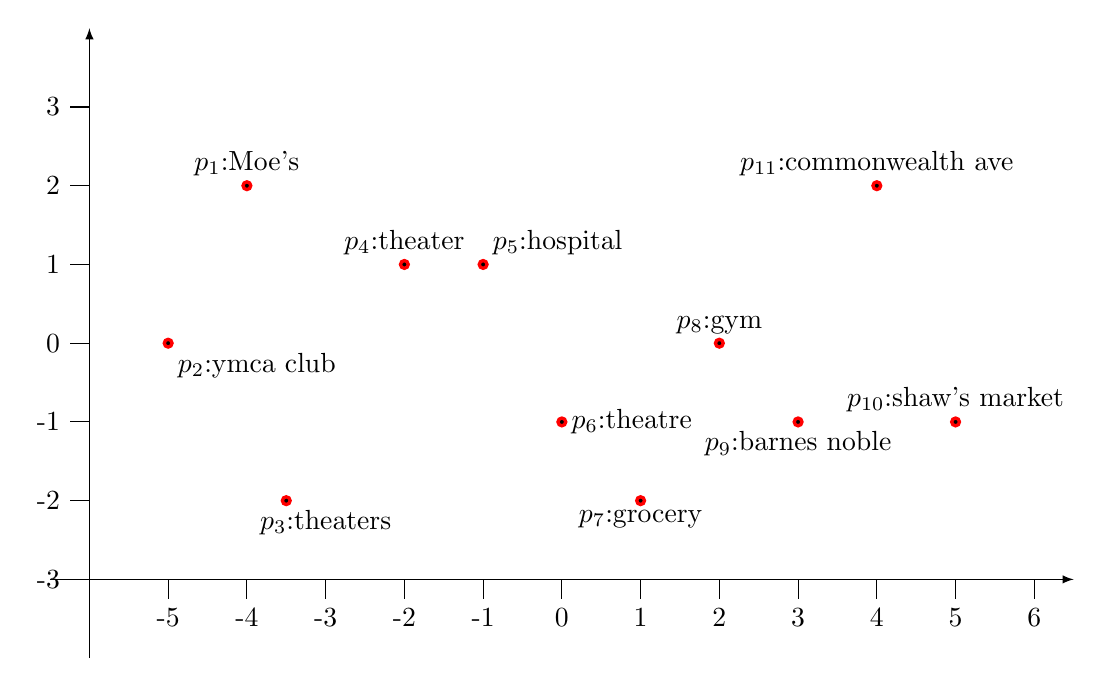
\begin{tikzpicture}
      % generate random points
      \pgfmathsetseed{1908} % init random with the year Voronoi published his paper ;)
      \def\pts{(0, -1), (2, 0), (1, -2), (3, -1), (4, 2), (5, -1), (-1, 1), (-2, 1), (-3.5, -2), (-4, 2), (-5, 0)}
      % \xintFor* #1 in {\xintSeq {1}{\n}} \do{
      %   \pgfmathsetmacro{\ptx}{.9*\maxxy*rand} % random x in [-.9\maxxy,.9\maxxy]
      %   \pgfmathsetmacro{\pty}{.9*\maxxy*rand} % random y in [-.9\maxxy,.9\maxxy]
      %   \edef\pts{\pts, (\ptx,\pty)} % stock the random point
      % }
    
      % draw the points and their cells
      \xintForpair #1#2 in \pts \do{
        \edef\pta{#1,#2}
        \begin{scope}
          \xintForpair \#3#4 in \pts \do{
            \edef\ptb{#3,#4}
            \ifx\pta\ptb\relax % check if (#1,#2) == (#3,#4) ?
              \tikzstyle{myclip}=[];
            \else
              \tikzstyle{myclip}=[clip];
            \fi;
            \path[myclip] (#3,#4) to[half plane] (#1,#2);
          }
          \clip (-\maxxy,-\maxy) rectangle (\maxxy,\maxy); % last clip
          \pgfmathsetmacro{\randhue}{rnd}
          \definecolor{randcolor}{hsb}{\randhue,.5,1}
          % \fill[randcolor] (#1,#2) circle (4*\biglen); % fill the cell with random color
          % \fill[fill={rgb:black,1;white,2}] (#1, #2) circle (4*\biglen);
          \fill[draw=red,very thick] (#1,#2) circle (1.4pt); % and draw the point
        \end{scope}
      }
      \pgfresetboundingbox
      % \draw (-\maxxy,-\maxy) rectangle (\maxxy,\maxy);
      % \draw[thick] (-5, 0) rectangle (-4, 2);
      % \draw[thick] (-3, -2) rectangle (-1, 1);
      % \draw[thick] (-5, -2) rectangle (-1, 2);
      % \draw[thick] (0, -2) rectangle (2, 0);
      % \draw[thick] (3, -2) rectangle (5, 2);
      % \draw[thick] (0, -2) rectangle (5, 2);
      \draw[-latex] (-6, -4) -- (-6, 4);
      \draw[-latex] (-6.5, -3) -- (6.5, -3);
      \foreach \i in {-5, -4,...,6}
      {
        \draw (\i, -3) -- (\i, -3.25) node[below] {\i};
      }
      \foreach \ii in {-3, -2,...,3}
      {
        \draw (-6, \ii) -- (-6.25, \ii) node[left] {\ii};
      }
      % \draw[very thick] (-0.5, 4) -- (-0.5, -4);
      \node[above] (p1) at (-4, 2) {$p_1$:Moe's};
      \node[below right] (p2) at (-5, 0) {$p_2$:ymca club};
      \node[below] (p3) at (-3, -2) {$p_3$:theaters};
      \node[above] (p4) at (-2, 1) {$p_4$:theater};
      \node[above right] (p5) at(-1, 1) {$p_5$:hospital};
      \node[right] (p6) at(0, -1){$p_6$:theatre};
      \node[below] (p7) at(1, -2){$p_7$:grocery};
      \node[above] (p8) at(2, 0) {$p_8$:gym};
      \node[below] (p9) at(3, -1){$p_9$:barnes noble};
      \node[above] (p10) at(5, -1) {$p_{10}$:shaw's market}; 
      \node[above] (p11) at(4, 2) {$p_{11}$:commonwealth ave};
    \end{tikzpicture}
    }
    \caption{原始数据} \label{fig:origin-data}
\end{figure}

\subsection{数据导入}
在进行数据划分前,首先对数据进行预处理,构造出$D$对应的Voronoi图,并将每个数据的邻居节点$VN(p_i)$和cell内包含的节点$V(p_i)$记录在叶子节点$p_i$上。
如对于$p_4$而言,其叶子节点中记录Voronoi图中的邻居$\{p_1, p_2, p_3, p_5, p_6\}$,所有的记录都是位置(在本例中即二维坐标)。
如图\ref{fig:pre-processing-data}所示。
\begin{figure}[H]
  \centering
  \resizebox{0.8\columnwidth}{!}{
  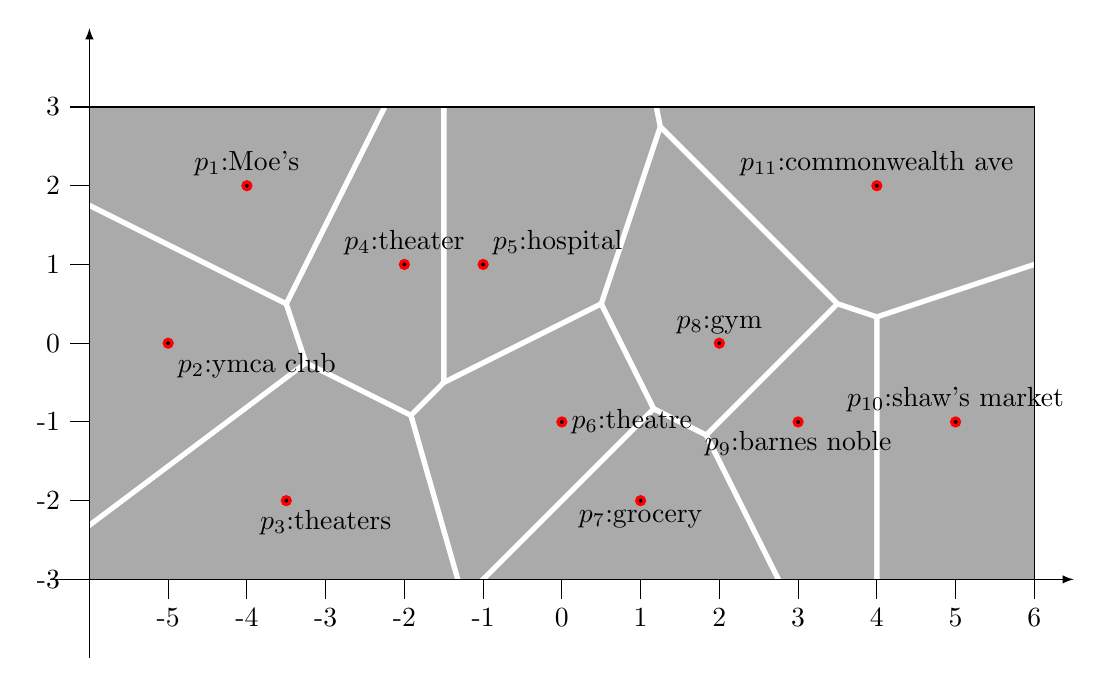
\begin{tikzpicture}
    % generate random points
    \pgfmathsetseed{1908} % init random with the year Voronoi published his paper ;)
    \def\pts{(0, -1), (2, 0), (1, -2), (3, -1), (4, 2), (5, -1), (-1, 1), (-2, 1), (-3.5, -2), (-4, 2), (-5, 0)}
    % \xintFor* #1 in {\xintSeq {1}{\n}} \do{
    %   \pgfmathsetmacro{\ptx}{.9*\maxxy*rand} % random x in [-.9\maxxy,.9\maxxy]
    %   \pgfmathsetmacro{\pty}{.9*\maxxy*rand} % random y in [-.9\maxxy,.9\maxxy]
    %   \edef\pts{\pts, (\ptx,\pty)} % stock the random point
    % }
  
    % draw the points and their cells
    \xintForpair #1#2 in \pts \do{
      \edef\pta{#1,#2}
      \begin{scope}
        \xintForpair \#3#4 in \pts \do{
          \edef\ptb{#3,#4}
          \ifx\pta\ptb\relax % check if (#1,#2) == (#3,#4) ?
            \tikzstyle{myclip}=[];
          \else
            \tikzstyle{myclip}=[clip];
          \fi;
          \path[myclip] (#3,#4) to[half plane] (#1,#2);
        }
        \clip (-\maxxy,-\maxy) rectangle (\maxxy,\maxy); % last clip
        \pgfmathsetmacro{\randhue}{rnd}
        \definecolor{randcolor}{hsb}{\randhue,.5,1}
        % \fill[randcolor] (#1,#2) circle (4*\biglen); % fill the cell with random color
        \fill[fill={rgb:black,1;white,2}] (#1, #2) circle (4*\biglen);
        \fill[draw=red,very thick] (#1,#2) circle (1.4pt); % and draw the point
      \end{scope}
    }
    \pgfresetboundingbox
    \draw (-\maxxy,-\maxy) rectangle (\maxxy,\maxy);
    % \draw[thick] (-5, 0) rectangle (-4, 2);
    % \draw[thick] (-3, -2) rectangle (-1, 1);
    % \draw[thick] (-5, -2) rectangle (-1, 2);
    % \draw[thick] (0, -2) rectangle (2, 0);
    % \draw[thick] (3, -2) rectangle (5, 2);
    % \draw[thick] (0, -2) rectangle (5, 2);
    \draw[-latex] (-6, -4) -- (-6, 4);
    \draw[-latex] (-6.5, -3) -- (6.5, -3);
    \foreach \i in {-5, -4,...,6}
    {
      \draw (\i, -3) -- (\i, -3.25) node[below] {\i};
    }
    \foreach \ii in {-3, -2,...,3}
    {
      \draw (-6, \ii) -- (-6.25, \ii) node[left] {\ii};
    }
    % \draw[very thick] (-0.5, 4) -- (-0.5, -4);
    \node[above] (p1) at (-4, 2) {$p_1$:Moe's};
    \node[below right] (p2) at (-5, 0) {$p_2$:ymca club};
    \node[below] (p3) at (-3, -2) {$p_3$:theaters};
    \node[above] (p4) at (-2, 1) {$p_4$:theater};
    \node[above right] (p5) at(-1, 1) {$p_5$:hospital};
    \node[right] (p6) at(0, -1){$p_6$:theatre};
    \node[below] (p7) at(1, -2){$p_7$:grocery};
    \node[above] (p8) at(2, 0) {$p_8$:gym};
    \node[below] (p9) at(3, -1){$p_9$:barnes noble};
    \node[above] (p10) at(5, -1) {$p_{10}$:shaw's market}; 
    \node[above] (p11) at(4, 2) {$p_{11}$:commonwealth ave};
  \end{tikzpicture}
  }
  \caption{数据预处理} \label{fig:pre-processing-data}
\end{figure}
利用\ref{sec:data-partition}节提到的数据划分策略,会选择在横坐标(方差更大)的中位数作为划分,默认中位数属于右侧,
则设定阈值$P_{max} = 6$,整体共有数据$11$个,可以得到示意性划分,如图\ref{fig:data-partition}所示,处在$DP$线两侧的数据各属一台机器,各自是一棵MVR-Tree。

\begin{figure}[H]
  \centering
  \resizebox{0.8\columnwidth}{!}{
  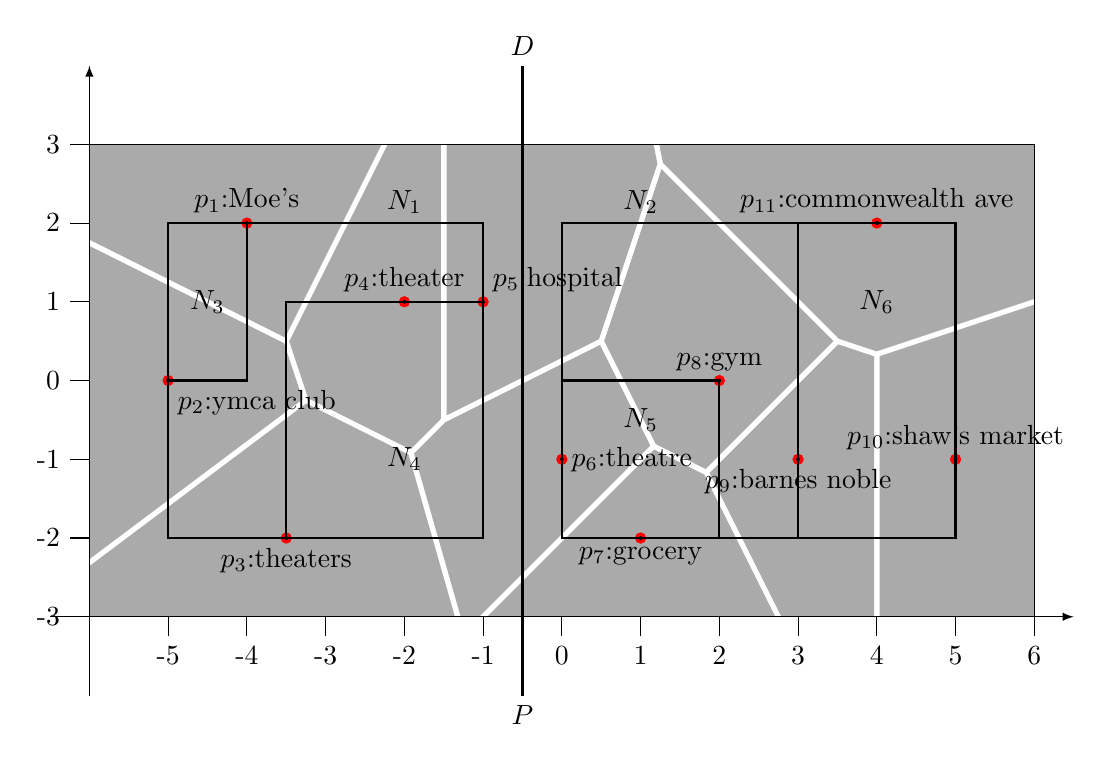
\begin{tikzpicture}
    % generate random points
    \pgfmathsetseed{1908} % init random with the year Voronoi published his paper ;)
    \def\pts{(0, -1), (2, 0), (1, -2), (3, -1), (4, 2), (5, -1), (-1, 1), (-2, 1), (-3.5, -2), (-4, 2), (-5, 0)}
    % \xintFor* #1 in {\xintSeq {1}{\n}} \do{
    %   \pgfmathsetmacro{\ptx}{.9*\maxxy*rand} % random x in [-.9\maxxy,.9\maxxy]
    %   \pgfmathsetmacro{\pty}{.9*\maxxy*rand} % random y in [-.9\maxxy,.9\maxxy]
    %   \edef\pts{\pts, (\ptx,\pty)} % stock the random point
    % }
  
    % draw the points and their cells
    \xintForpair #1#2 in \pts \do{
      \edef\pta{#1,#2}
      \begin{scope}
        \xintForpair \#3#4 in \pts \do{
          \edef\ptb{#3,#4}
          \ifx\pta\ptb\relax % check if (#1,#2) == (#3,#4) ?
            \tikzstyle{myclip}=[];
          \else
            \tikzstyle{myclip}=[clip];
          \fi;
          \path[myclip] (#3,#4) to[half plane] (#1,#2);
        }
        \clip (-\maxxy,-\maxy) rectangle (\maxxy,\maxy); % last clip
        \pgfmathsetmacro{\randhue}{rnd}
        \definecolor{randcolor}{hsb}{\randhue,.5,1}
        % \fill[randcolor] (#1,#2) circle (4*\biglen); % fill the cell with random color
        \fill[fill={rgb:black,1;white,2}] (#1, #2) circle (4*\biglen);
        \fill[draw=red,very thick] (#1,#2) circle (1.4pt); % and draw the point
      \end{scope}
    }
    \pgfresetboundingbox
    \draw (-\maxxy,-\maxy) rectangle (\maxxy,\maxy);
    \draw[thick] (-5, 0) rectangle (-4, 2);
    \draw[thick] (-3.5, -2) rectangle (-1, 1);
    \draw[thick] (-5, -2) rectangle (-1, 2);
    \draw[thick] (0, -2) rectangle (2, 0);
    \draw[thick] (3, -2) rectangle (5, 2);
    \draw[thick] (0, -2) rectangle (5, 2);
    \draw[-latex] (-6, -4) -- (-6, 4);
    \draw[-latex] (-6.5, -3) -- (6.5, -3);
    \foreach \i in {-5, -4,...,6}
    {
      \draw (\i, -3) -- (\i, -3.25) node[below] {\i};
    }
    \foreach \ii in {-3, -2,...,3}
    {
      \draw (-6, \ii) -- (-6.25, \ii) node[left] {\ii};
    }
    \draw[very thick] (-0.5, 4) -- (-0.5, -4);
    \node[below] (data-partition-1) at (-0.5, -4) {$P$};
    \node[above] (data-partition-2) at (-0.5, 4) {$D$};
    \node[above] (p1) at (-4, 2) {$p_1$:Moe's};
    \node[below right] (p2) at (-5, 0) {$p_2$:ymca club};
    \node[below] (p3) at (-3.5, -2) {$p_3$:theaters};
    \node[above] (p4) at (-2, 1) {$p_4$:theater};
    \node[above right] (p5) at(-1, 1) {$p_5$:hospital};
    \node[right] (p6) at(0, -1){$p_6$:theatre};
    \node[below] (p7) at(1, -2){$p_7$:grocery};
    \node[above] (p8) at(2, 0) {$p_8$:gym};
    \node[below] (p9) at(3, -1){$p_9$:barnes noble};
    \node[above] (p10) at(5, -1) {$p_{10}$:shaw's market}; 
    \node[above] (p11) at(4, 2) {$p_{11}$:commonwealth ave};
    \node[above] (n1) at (-2, 2) {$N_1$};
    \node[above] (n2) at (1, 2) {$N_2$};
    \node (n3) at (-4.5, 1) {$N_3$};
    \node (n4) at (-2, -1) {$N_4$};
    \node (n5) at (1, -0.5) {$N_5$};
    \node (n6) at (4, 1) {$N_6$};
  \end{tikzpicture}
  }
  \caption{数据划分与索引构建} \label{fig:data-partition}
\end{figure}

\subsection{查询处理}
\subsubsection{Range Query处理}
以图\ref{fig:range-query-example}为例,当查询$Q = (r, \{(theatre, 2)\})$来到时,首先确定查询范围与有交集的
机器,并将查询发往相应的机器上。在本例中,$Q$会发往$N_1$和$N_2$两台机器。此后,就进入本地的查询即可。

在$N_1$上查询,判断其两个儿子$N3, N_4$的MBR与查询范围$r$判断是否存在交集,
显然可以将$N_3$剪枝掉,查询进入$N_4$。再依次将$N_4$的儿子节点$p_4, p_5, p_3$加入队列,
其中$p_3$在$r$之外,直接剪枝。依次判断$p_4$,与关键字的编辑距离恰好为$2$,输出$p_4$。
在$N_2$机器上的查询与此过程类似。

\begin{figure}[H]
  \centering
  \resizebox{0.8\columnwidth}{!}{
  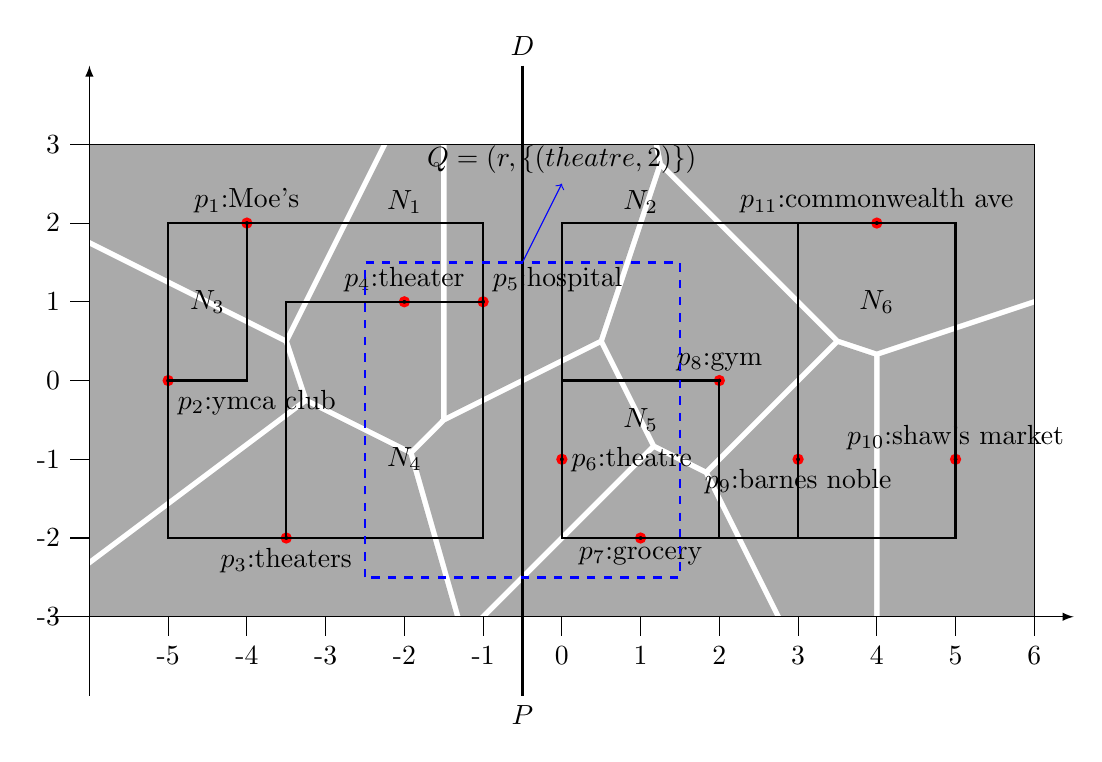
\begin{tikzpicture}
    % generate random points
    \pgfmathsetseed{1908} % init random with the year Voronoi published his paper ;)
    \def\pts{(0, -1), (2, 0), (1, -2), (3, -1), (4, 2), (5, -1), (-1, 1), (-2, 1), (-3.5, -2), (-4, 2), (-5, 0)}
    % \xintFor* #1 in {\xintSeq {1}{\n}} \do{
    %   \pgfmathsetmacro{\ptx}{.9*\maxxy*rand} % random x in [-.9\maxxy,.9\maxxy]
    %   \pgfmathsetmacro{\pty}{.9*\maxxy*rand} % random y in [-.9\maxxy,.9\maxxy]
    %   \edef\pts{\pts, (\ptx,\pty)} % stock the random point
    % }
  
    % draw the points and their cells
    \xintForpair #1#2 in \pts \do{
      \edef\pta{#1,#2}
      \begin{scope}
        \xintForpair \#3#4 in \pts \do{
          \edef\ptb{#3,#4}
          \ifx\pta\ptb\relax % check if (#1,#2) == (#3,#4) ?
            \tikzstyle{myclip}=[];
          \else
            \tikzstyle{myclip}=[clip];
          \fi;
          \path[myclip] (#3,#4) to[half plane] (#1,#2);
        }
        \clip (-\maxxy,-\maxy) rectangle (\maxxy,\maxy); % last clip
        \pgfmathsetmacro{\randhue}{rnd}
        \definecolor{randcolor}{hsb}{\randhue,.5,1}
        % \fill[randcolor] (#1,#2) circle (4*\biglen); % fill the cell with random color
        \fill[fill={rgb:black,1;white,2}] (#1, #2) circle (4*\biglen);
        \fill[draw=red,very thick] (#1,#2) circle (1.4pt); % and draw the point
      \end{scope}
    }
    \pgfresetboundingbox
    \draw (-\maxxy,-\maxy) rectangle (\maxxy,\maxy);
    \draw[thick] (-5, 0) rectangle (-4, 2);
    \draw[thick] (-3.5, -2) rectangle (-1, 1);
    \draw[thick] (-5, -2) rectangle (-1, 2);
    \draw[thick] (0, -2) rectangle (2, 0);
    \draw[thick] (3, -2) rectangle (5, 2);
    \draw[thick] (0, -2) rectangle (5, 2);
    \draw[-latex] (-6, -4) -- (-6, 4);
    \draw[-latex] (-6.5, -3) -- (6.5, -3);
    \foreach \i in {-5, -4,...,6}
    {
      \draw (\i, -3) -- (\i, -3.25) node[below] {\i};
    }
    \foreach \ii in {-3, -2,...,3}
    {
      \draw (-6, \ii) -- (-6.25, \ii) node[left] {\ii};
    }
    \draw[very thick] (-0.5, 4) -- (-0.5, -4);
    \node[above] (p1) at (-4, 2) {$p_1$:Moe's};
    \node[below right] (p2) at (-5, 0) {$p_2$:ymca club};
    \node[below] (p3) at (-3.5, -2) {$p_3$:theaters};
    \node[above] (p4) at (-2, 1) {$p_4$:theater};
    \node[above right] (p5) at(-1, 1) {$p_5$:hospital};
    \node[right] (p6) at(0, -1){$p_6$:theatre};
    \node[below] (p7) at(1, -2){$p_7$:grocery};
    \node[above] (p8) at(2, 0) {$p_8$:gym};
    \node[below] (p9) at(3, -1){$p_9$:barnes noble};
    \node[above] (p10) at(5, -1) {$p_{10}$:shaw's market}; 
    \node[above] (p11) at(4, 2) {$p_{11}$:commonwealth ave};
    \draw[thick, dashed, blue] (-2.5, -2.5) rectangle (1.5, 1.5);
    \draw[->, blue] (-0.5, 1.5) -- (0, 2.5);
    \node[above] (n1) at (-2, 2) {$N_1$};
    \node[above] (n2) at (1, 2) {$N_2$};
    \node (n3) at (-4.5, 1) {$N_3$};
    \node (n4) at (-2, -1) {$N_4$};
    \node (n5) at (1, -0.5) {$N_5$};
    \node (n6) at (4, 1) {$N_6$};
    \node[below] (data-partition-1) at (-0.5, -4) {$P$};
    \node[above] (data-partition-2) at (-0.5, 4) {$D$};
    \node[above] (query) at (0, 2.5) {$\bm{Q = (r, \{(theatre, 2)\})}$};
  \end{tikzpicture}
  }
  \caption{Range Query示例}\label{fig:range-query-example}
\end{figure}

\subsubsection{$k$NN查询处理}
对于$k$NN查询$q$,首先系统会使用全局索引根据其位置将其定位到某台机器,在本例中根据$q$的位置$r_q$会将其定位到$DP$左侧的机器上,
并将查询发往对应机器的MVR-Tree根节点$N_1$,$N_1$利用\ref{sec:algo-knn}节提到的算法,将$(N_4, 0), (N_3, 2)$插入堆中。
将堆顶元素$(N_4, 0)$弹出,将其子节点$(p_4, 1), (p_5, 1.414), (p_3, 2.5)$压入堆中。
再将堆顶元素$(p_4, 1)$弹出,\textbf{判断恰好$r_q$位于$p_4$所处的cell中,故$p_4$为$q$的$1$NN结果}。

将堆弹空,$p_4$的邻居压入堆$(p_5, 1.141), (p_6, 2.236), (p_3, 2.5)$,依次判断堆顶元素是否满足关键字编辑距离的阈值要求。
$p_5$不符合,继续判断堆顶此时发现$p_6$不在本机器上,故将堆内元素和当前的$counter$发往$p_6$所在机器。
在右侧继续执行$k$NN查询,\textbf{此时$p_6$符合编辑距离要求,输出$p_6$,$2$NN过程结束}。
\begin{figure}[H]
  \centering
  \resizebox{0.8\columnwidth}{!}{
  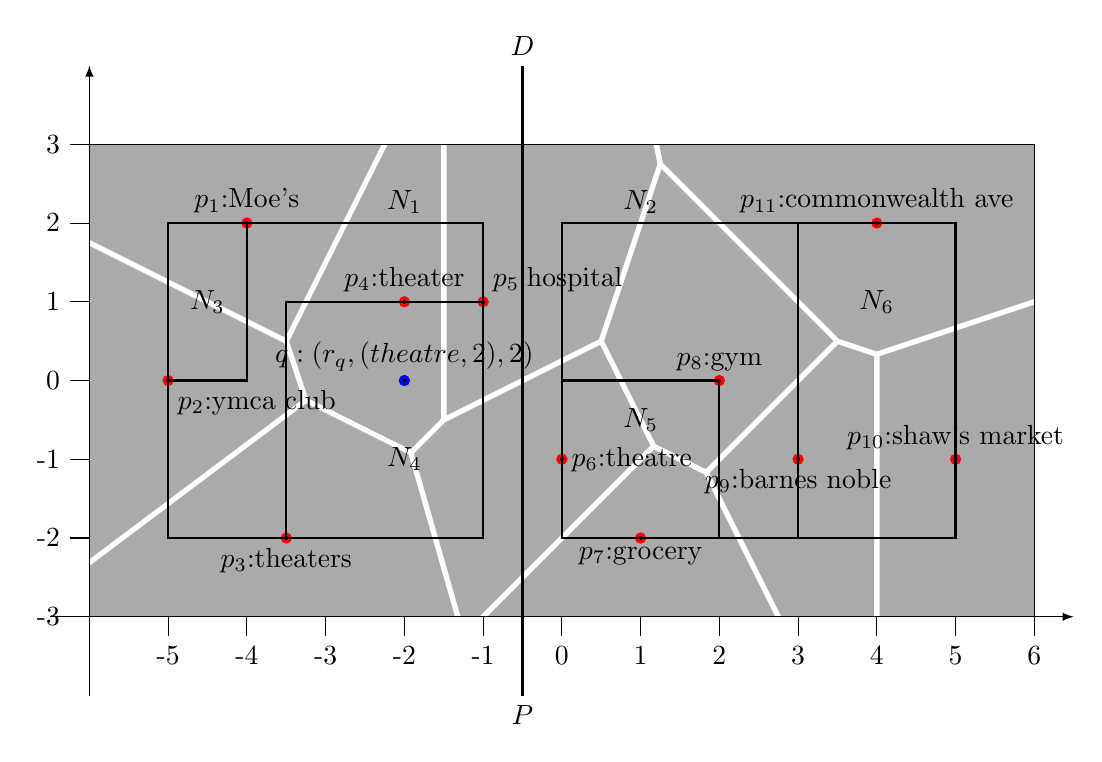
\begin{tikzpicture}
    % generate random points
    \pgfmathsetseed{1908} % init random with the year Voronoi published his paper ;)
    \def\pts{(0, -1), (2, 0), (1, -2), (3, -1), (4, 2), (5, -1), (-1, 1), (-2, 1), (-3.5, -2), (-4, 2), (-5, 0)}
    % \xintFor* #1 in {\xintSeq {1}{\n}} \do{
    %   \pgfmathsetmacro{\ptx}{.9*\maxxy*rand} % random x in [-.9\maxxy,.9\maxxy]
    %   \pgfmathsetmacro{\pty}{.9*\maxxy*rand} % random y in [-.9\maxxy,.9\maxxy]
    %   \edef\pts{\pts, (\ptx,\pty)} % stock the random point
    % }
  
    % draw the points and their cells
    \xintForpair #1#2 in \pts \do{
      \edef\pta{#1,#2}
      \begin{scope}
        \xintForpair \#3#4 in \pts \do{
          \edef\ptb{#3,#4}
          \ifx\pta\ptb\relax % check if (#1,#2) == (#3,#4) ?
            \tikzstyle{myclip}=[];
          \else
            \tikzstyle{myclip}=[clip];
          \fi;
          \path[myclip] (#3,#4) to[half plane] (#1,#2);
        }
        \clip (-\maxxy,-\maxy) rectangle (\maxxy,\maxy); % last clip
        \pgfmathsetmacro{\randhue}{rnd}
        \definecolor{randcolor}{hsb}{\randhue,.5,1}
        % \fill[randcolor] (#1,#2) circle (4*\biglen); % fill the cell with random color
        \fill[fill={rgb:black,1;white,2}] (#1, #2) circle (4*\biglen);
        \fill[draw=red,very thick] (#1,#2) circle (1.4pt); % and draw the point
      \end{scope}
    }
    \pgfresetboundingbox
    \draw (-\maxxy,-\maxy) rectangle (\maxxy,\maxy);
    \draw[thick] (-5, 0) rectangle (-4, 2);
    \draw[thick] (-3.5, -2) rectangle (-1, 1);
    \draw[thick] (-5, -2) rectangle (-1, 2);
    \draw[thick] (0, -2) rectangle (2, 0);
    \draw[thick] (3, -2) rectangle (5, 2);
    \draw[thick] (0, -2) rectangle (5, 2);
    \draw[-latex] (-6, -4) -- (-6, 4);
    \draw[-latex] (-6.5, -3) -- (6.5, -3);
    \foreach \i in {-5, -4,...,6}
    {
      \draw (\i, -3) -- (\i, -3.25) node[below] {\i};
    }
    \foreach \ii in {-3, -2,...,3}
    {
      \draw (-6, \ii) -- (-6.25, \ii) node[left] {\ii};
    }
    \draw[very thick] (-0.5, 4) -- (-0.5, -4);
    \node[above] (p1) at (-4, 2) {$p_1$:Moe's};
    \node[below right] (p2) at (-5, 0) {$p_2$:ymca club};
    \node[below] (p3) at (-3.5, -2) {$p_3$:theaters};
    \node[above] (p4) at (-2, 1) {$p_4$:theater};
    \node[above right] (p5) at(-1, 1) {$p_5$:hospital};
    \node[right] (p6) at(0, -1){$p_6$:theatre};
    \node[below] (p7) at(1, -2){$p_7$:grocery};
    \node[above] (p8) at(2, 0) {$p_8$:gym};
    \node[below] (p9) at(3, -1){$p_9$:barnes noble};
    \node[above] (p10) at(5, -1) {$p_{10}$:shaw's market}; 
    \node[above] (p11) at(4, 2) {$p_{11}$:commonwealth ave};
    \node[above] (q) at (-2, 0) {$\bm{q:(r_q, (theatre,2), 2)}$};
    \fill[draw=blue,very thick] (-2, 0) circle (1.4pt);
    \node[above] (n1) at (-2, 2) {$N_1$};
    \node[above] (n2) at (1, 2) {$N_2$};
    \node (n3) at (-4.5, 1) {$N_3$};
    \node (n4) at (-2, -1) {$N_4$};
    \node (n5) at (1, -0.5) {$N_5$};
    \node (n6) at (4, 1) {$N_6$};
    \node[below] (data-partition-1) at (-0.5, -4) {$P$};
    \node[above] (data-partition-2) at (-0.5, 4) {$D$};
  \end{tikzpicture}
  }
  \caption{$k$NN示例}\label{fig:knn-example}
\end{figure}

\subsection{R$k$NN示例}
\begin{figure}[H]
  \centering
  \resizebox{0.8\columnwidth}{!}{
  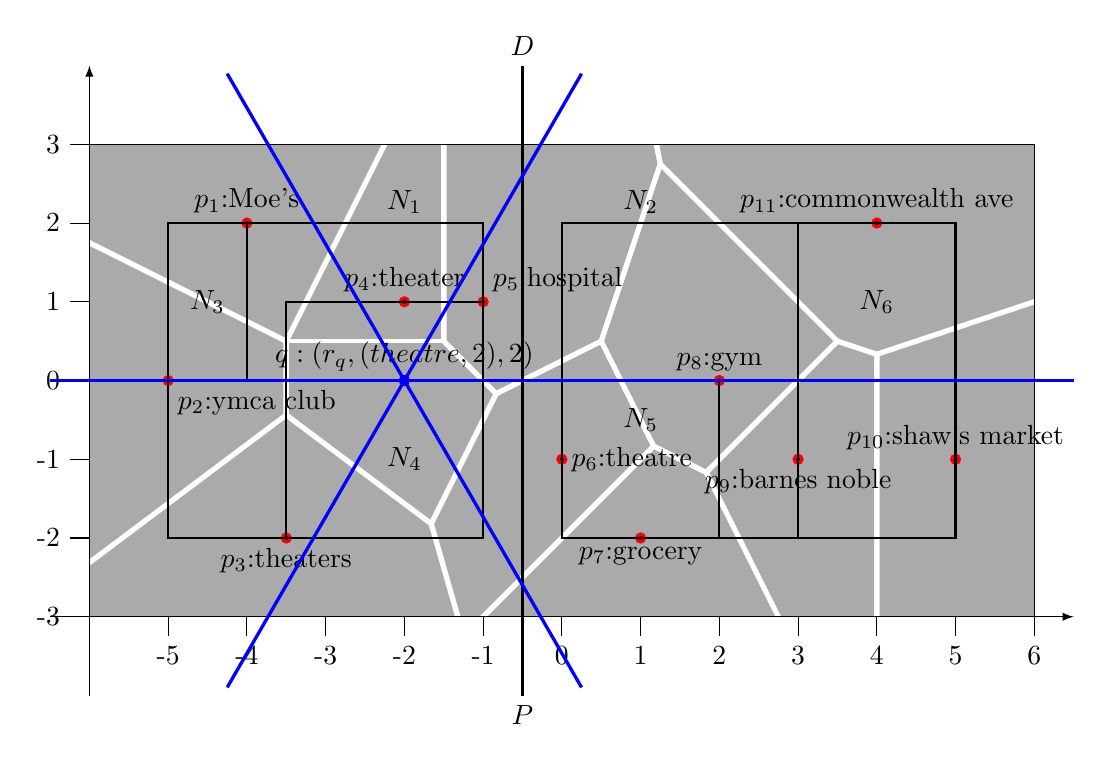
\begin{tikzpicture}
    \coordinate (q-center) at (-2,0);
    % generate random points
    \pgfmathsetseed{1908} % init random with the year Voronoi published his paper ;)
    \def\pts{(0, -1), (2, 0), (1, -2), (3, -1), (4, 2), (5, -1), (-1, 1), (-2, 1), (-3.5, -2), (-4, 2), (-5, 0), (-2, 0)}
    % \xintFor* #1 in {\xintSeq {1}{\n}} \do{
    %   \pgfmathsetmacro{\ptx}{.9*\maxxy*rand} % random x in [-.9\maxxy,.9\maxxy]
    %   \pgfmathsetmacro{\pty}{.9*\maxxy*rand} % random y in [-.9\maxxy,.9\maxxy]
    %   \edef\pts{\pts, (\ptx,\pty)} % stock the random point
    % }
  
    % draw the points and their cells
    \xintForpair #1#2 in \pts \do{
      \edef\pta{#1,#2}
      \begin{scope}
        \xintForpair \#3#4 in \pts \do{
          \edef\ptb{#3,#4}
          \ifx\pta\ptb\relax % check if (#1,#2) == (#3,#4) ?
            \tikzstyle{myclip}=[];
          \else
            \tikzstyle{myclip}=[clip];
          \fi;
          \path[myclip] (#3,#4) to[half plane] (#1,#2);
        }
        \clip (-\maxxy,-\maxy) rectangle (\maxxy,\maxy); % last clip
        \pgfmathsetmacro{\randhue}{rnd}
        \definecolor{randcolor}{hsb}{\randhue,.5,1}
        % \fill[randcolor] (#1,#2) circle (4*\biglen); % fill the cell with random color
        \fill[fill={rgb:black,1;white,2}] (#1, #2) circle (4*\biglen);
        \fill[draw=red,very thick] (#1,#2) circle (1.4pt); % and draw the point
      \end{scope}
    }
    \pgfresetboundingbox
    \draw (-\maxxy,-\maxy) rectangle (\maxxy,\maxy);
    \draw[thick] (-5, 0) rectangle (-4, 2);
    \draw[thick] (-3.5, -2) rectangle (-1, 1);
    \draw[thick] (-5, -2) rectangle (-1, 2);
    \draw[thick] (0, -2) rectangle (2, 0);
    \draw[thick] (3, -2) rectangle (5, 2);
    \draw[thick] (0, -2) rectangle (5, 2);
    \draw[-latex] (-6, -4) -- (-6, 4);
    \draw[-latex] (-6.5, -3) -- (6.5, -3);
    \foreach \i in {-5, -4,...,6}
    {
      \draw (\i, -3) -- (\i, -3.25) node[below] {\i};
    }
    \foreach \ii in {-3, -2,...,3}
    {
      \draw (-6, \ii) -- (-6.25, \ii) node[left] {\ii};
    }
    \draw[very thick] (-0.5, 4) -- (-0.5, -4);
    \node[above] (p1) at (-4, 2) {$p_1$:Moe's};
    \node[below right] (p2) at (-5, 0) {$p_2$:ymca club};
    \node[below] (p3) at (-3.5, -2) {$p_3$:theaters};
    \node[above] (p4) at (-2, 1) {$p_4$:theater};
    \node[above right] (p5) at(-1, 1) {$p_5$:hospital};
    \node[right] (p6) at(0, -1){$p_6$:theatre};
    \node[below] (p7) at(1, -2){$p_7$:grocery};
    \node[above] (p8) at(2, 0) {$p_8$:gym};
    \node[below] (p9) at(3, -1){$p_9$:barnes noble};
    \node[above] (p10) at(5, -1) {$p_{10}$:shaw's market}; 
    \node[above] (p11) at(4, 2) {$p_{11}$:commonwealth ave};
    \node[above] (q) at (-2, 0) {$\bm{q:(r_q, (theatre,2), 2)}$};
    \fill[draw=blue,very thick] (-2, 0) circle (1.4pt);
    \node[above] (n1) at (-2, 2) {$N_1$};
    \node[above] (n2) at (1, 2) {$N_2$};
    \node (n3) at (-4.5, 1) {$N_3$};
    \node (n4) at (-2, -1) {$N_4$};
    \node (n5) at (1, -0.5) {$N_5$};
    \node (n6) at (4, 1) {$N_6$};
    \node[below] (data-partition-1) at (-0.5, -4) {$P$};
    \node[above] (data-partition-2) at (-0.5, 4) {$D$};
    \draw[blue, very thick] (q-center.60) -- ++(60:4.5);
    \draw[blue, very thick] (q-center.0) -- ++(0:8.5);
    \draw[blue, very thick] (q-center.120) -- ++(120:4.5);
    \draw[blue, very thick] (q-center.180) -- ++(180:4.5);
    \draw[blue, very thick] (q-center.240) -- ++(240:4.5);
    \draw[blue, very thick] (q-center.300) -- ++(300:4.5);
  \end{tikzpicture}
  }
  \caption{R$k$NN示例}\label{fig:Rknn-example}
\end{figure}
% \section{实验心得}
\appendix

% \section{参考文献}
\begin{thebibliography}{20}
    \bibitem{R-Tree} Guttman A. R-trees: a dynamic index structure for spatial searching[M]. ACM, 1984.
    \bibitem{Voronoi-Diagram} Aurenhammer F. Voronoi diagrams—a survey of a fundamental geometric data structure[J]. ACM Computing Surveys (CSUR), 1991, 23(3): 345-405.
    \bibitem{6-partitions} Stanoi I, Agrawal D, El Abbadi A. Reverse nearest neighbor queries for dynamic databases[C]//ACM SIGMOD workshop on research issues in data mining and knowledge discovery. 2000: 44-53.
    \bibitem{TPL} Tao Y, Papadias D, Lian X. Reverse kNN search in arbitrary dimensionality[C]//Proceedings of the Thirtieth international conference on Very large data bases-Volume 30. VLDB Endowment, 2004: 744-755.
    \bibitem{VD-Property} Okabe A, Boots B, Sugihara K, et al. Spatial tessellations: concepts and applications of Voronoi diagrams[M]. John Wiley \& Sons, 2009.
    \bibitem{VoR-Tree} Sharifzadeh M, Shahabi C. Vor-tree: R-trees with voronoi diagrams for efficient processing of spatial nearest neighbor queries[J]. Proceedings of the VLDB Endowment, 2010, 3(1-2): 1231-1242.
    \bibitem{RT-CAN} Wang J, Wu S, Gao H, et al. Indexing multi-dimensional data in a cloud system[C]//Proceedings of the 2010 ACM SIGMOD International Conference on Management of data. ACM, 2010: 591-602.
    \bibitem{MHR-Tree} Li F, Yao B, Tang M, et al. Spatial approximate string search[J]. IEEE Transactions on Knowledge and Data Engineering, 2012, 25(6): 1394-1409.
    \bibitem{KD-Tree-Partition} Mishra S, Suman A C. An efficient method of partitioning high volumes of multidimensional data for parallel clustering algorithms[J]. arXiv preprint arXiv:1609.06221, 2016.
\end{thebibliography}

\end{document}
